\newcommand{\ClassPath}{../../VIU_TFM_LaTeX_template}
\documentclass{\ClassPath/viu-tfm-template}
\usepackage{multicol}

\definecolor{maincolor}{HTML}{f25416}

%--------------------------------------------------------------------------
% Definiciones necesarias Modifica con tus datos
%--------------------------------------------------------------------------
\def\nombre{Gómez Olivencia, Rubén}
\def\dni{78910013-A}
\def\titulo{Aplicación Android hecha en Kotlin \linebreak\linebreak con gestión de dependencias, \linebreak\linebreak acceso a internet y guardado de datos }
\def\titulacion{Máster Universitario en Desarrollo de Aplicaciones y Servicios Web}
\def\curso{2022-2023}

%Los siguientes son opcionales: si no se ponen, la portada cambia un poco. Ideal para escribir artículos/trabajos cortos
\def\dirige{}
\def\convocatoria{}
\def\asignatura{Programación en dispositivos móviles (wearables)}


% importar fichero de Bibliografía
%\addbibresource{Actividad_1.bib}

\begin{document}
    \graphicspath{{../../VIU_TFM_LaTeX_template/}}

    \coverpage

    \tableofcontents

\chapter{Introducción}

A la hora de crear una aplicación de móvil moderna podemos utilizar como fuente de inspiración cualquiera de las que utilizamos en nuestro día a día.

Si realizamos un pequeño análisis de las mismas, veremos que todas ellas hacen uso de la conectividad de red para obtener (o enviar) datos a internet, y que parte de esos datos serán almacenados en una base de datos interna en el propio móvil.

En esta documentación se va a explicar los pasos realizados para la creación de una aplicación que funcionará en el sistema operativo Android y creada bajo el lenguaje de programación Kotlin, la cual hará uso de un sistema de inyección de dependenciasm, acceso a internet y gestión de una base de datos propia.


\chapter{Requisitos del proyecto}

Como todo proyecto, debemos ceñirnos a unos requisitos que asegurarán que el resultado final cumple con las expectativas esperadas. En este caso, el objetivo es profundizar en ciertas características que cualquier aplicación moderna para Android cumple a día de hoy.

Los requisitos establecidos son:

\begin{itemize}
    \item Obtener un listado de películas de un servicio HTTPS, que recibirá un fichero JSON. Para ello se utilizará la librería \href{https://github.com/square/retrofit}{retrofit}.
    \item Se creará un modelo de datos para el correcto \textit{parseo} de los datos recibidos.
    \item Estos datos se guardarán en una base de datos interna en el móvil utilizando \href{https://developers.google.com/protocol-buffers}{Protocol Buffers} y \href{https://developer.android.com/topic/libraries/architecture/datastore}{DataStore}. Se podrán eliminar las películas de la base de datos.
    \item La visualización de los datos se hará mediante el componente \href{https://developer.android.com/develop/ui/views/layout/recyclerview}{RecyclerView}.
    \item Al seleccionar una película del listado, nos enviará a otra pantalla para ver más información de la misma.
    \item Se debe hacer uso de un sistema de inyección de dependencias, como por ejemplo \href{https://insert-koin.io/}{Koin}.
\end{itemize}


\chapter{Creación del proyecto}

Para la creación del proyecto se ha hecho uso del entorno de desarrollo \href{https://developer.android.com/studio/}{Android Studio}, que es el IDE oficial que nos permite programar teniendo todos los recursos necesarios.

Por otro lado, se ha hecho uso del lenguaje de programación \href{https://kotlinlang.org/}{Kotlin}, ya que desde el año 2019 Google lo ha puesto como el lenguaje de programación preferido a la hora de realizar los desarrollos para la plataforma Android.

A continuación se detallan los aspectos más destacados del proyecto.

\section{Inyección de dependencias}
A la hora de crear un proyecto es posible que utilicemos distintos componentes o clases que se referencien unos de otros. Para facilitar que estas referencias se cumplan se hará uso de la inyección de dependencias utilizando la librería \href{https://insert-koin.io/}{Koin}.


\begin{mycode}{Inicialización de Koin en App.kt}{XML}{}
startKoin {
    androidLogger(Level.ERROR)
    androidContext(this@App)
    modules(
        module { single { moviesDataStore } },
        mainModule,
        mainActivity
    )
}
\end{mycode}

Aunque no es obligatorio el uso de librerías externas para la inyección de dependencias, Koin nos va a ayudar asegurando que lo realizamos de forma correcta y de esta manera evitaremos bugs de implementación.

\section{Conexión a internet y obtención de datos}
La gran mayoría de aplicaciones que utilizamos hoy en día hacen uso de conexión a internet, por lo que es necesario entender cómo funciona este sistema dentro del ecosistema Android.

En primer lugar la aplicación debe de contar con los permisos necesarios para poder acceder a internet. Para ellos se deben especificar los permisos en el fichero \configfile{AndroidManifest.xml}


\begin{mycode}{Permisos de red en AndroidManifest.xml}{XML}{{\small }}
<uses-permission android:name="android.permission.INTERNET" />
<uses-permission android:name="android.permission.ACCESS_NETWORK_STATE" />
\end{mycode}

Con los permisos configurados es momento de saber cómo realizar la conexión para obtener ficheros y/o información. En nuestro caso se va a utilizar la librería \href{https://github.com/square/retrofit}{retrofit} para la descarga de un fichero \href{https://gist.githubusercontent.com/skydoves/176c209dbce4a53c0ff9589e07255f30/raw/6489d9712702e093c4df71500fb822f0d408ef75/DisneyPosters2.json}{json} que contiene un listado de películas.

La configuración cuenta con varias partes:
\begin{itemize}
    \item Construcción de la instancia del servidor, en la que indicamos cuál es el servidor al que vamos a conectarnos
    \begin{mycode}{Instancia de Retrofit}{kotlin}{}
Retrofit.Builder()
    .baseUrl("https://gist.githubusercontent.com/")
    .addConverterFactory(
        MoshiConverterFactory.create(
            Moshi.Builder()
              .add(KotlinJsonAdapterFactory())
              .build()
        )
    )
    .build()
    .create(MoviesInterface::class.java)
    \end{mycode}

    \item Interfaz de conexión, en la que se indica el resto de la URL a la que queremos acceder.
    \begin{mycode}{Interfaz Retrofit en MoviesInterface.kt}{kotlin}{}
package com.rugoli.moviedb.interfaces
import retrofit2.http.GET
interface MoviesInterface {
    // URL cortada
    @GET("skydoves/.../DisneyPosters2.json")
    suspend fun downloadMovies():
        List<com.rugoli.moviedb.dataclass.Movie>
}
\end{mycode}

    \item Junto con el código anterior, se indica que el resultado obtenido se va a parsear para obtener una lista de objetos “Movie”, que está especificado dentro del paquete \textbf{dataclass.Movie}. En este fichero se indica cómo es la clase y los distintos atributos que contiene.

    \item Ya sólo queda realizar la llamada para obtener los datos, que en este caso se hace desde el modelo de datos, que posteriormente se explicará con más detalle.
\end{itemize}

Con lo explicado la aplicación es capaz de realizar la descarga del fichero, parsear el json obtenido y crear un listado de objetos de una clase propia. De esta manera los datos se podrán utilizar posteriormente.


\section{Data Store y Protocol Buffers}
Una vez sabemos cómo realizar la descarga de datos, el siguiente paso es almacenarlos.

Es importante entender que \textbf{Data Store} se puede utilizar con datos estructurados y con datos en formato “clave-valor”. El primer caso es habitual utilizarlo como si fuese una base de datos SQL, mientras que el uso de “clave-valor” es más habitual si sólo queremos guardar configuración de la aplicación.

En nuestro caso, que vamos a utilizar datos estructurados, vamos a diferenciar el desarrollo en dos apartados:
\begin{itemize}
    \item Estructurar los datos
    \item Guardar y recuperar los datos
\end{itemize}


\subsection{Estructurar los datos}
En el caso que nos ocupa, se va a crear una estructura de datos que forma la película (con los datos descargados), para posteriormente almacenarlos. Para realizar esta estructura se va a utilizar \href{https://developers.google.com/protocol-buffers}{Protocol Buffers}.

La configuración está dividida en distintos apartados que detallaremos a continuación:
\begin{itemize}
    \item Hay que indicar que se va a utilizar Protocol Buffers, para ello se configura \configfile{build.gradle}

    \item \textbf{Estructura de los datos}, dentro del fichero de configuración \configfile{proto/movie.proto}. Este fichero sería el equivalente a un “\textit{schema}” de creación de una tabla en MySQL.

    \item Creación de un \textbf{\textit{Serializer}} que le indica a Datastore cómo leer y escribir el tipo de datos. Está creado en el fichero \configfile{MovieStoreSerializer.kt}
\end{itemize}


\subsection{Guardar, recuperar y borrar los datos}

Antes de comenzar a guardar y recuperar datos, en la aplicación debemos indicar que vamos a hacer uso de DataStore y su configuración (indicando el fichero que debe crear y el \textit{Serializer} a utilizar)

\begin{mycode}{Creamos variable global para Datastore en App.kt}{kotlin}{}
private val moviesDataStore: DataStore<MovieStore> by dataStore(
    fileName = "movies.pb",
    serializer = MovieStoreSerializer
)
\end{mycode}

Tras esto, hay que decidir dónde se va a hacer uso de los datos, y para ello se ha creado el modelo de datos \textbf{Movie} dentro del fichero \configfile{models/Movie.kt}. Este modelo de datos se encarga de:

\begin{itemize}
    \item \textbf{Guardar los datos} en el DataStore. Dependiendo de si la base de datos está vacía (ya sea porque es la primera vez que se ejecuta la aplicación o porque se han borrado todos los datos), descargará los datos de internet.
\begin{mycode}{Guardamos los datos con Datastore}{kotlin}{}
if (isInitialized == false) {
    moviesDataStore.updateData { movieStore ->
        movieStore.toBuilder()
        .addAllMovies(moviesToStore)
        .setInitialized(true)
        .build()
    }
}
\end{mycode}
    \item \textbf{Recuperar los datos} al iniciar la aplicación. De esta manera se creará el RecyclerView que veremos posteriormente.

    \item \textbf{Borrado de datos} al pulsar el icono de borrado/papelera que se encuentra junto a una película.
\end{itemize}


\section{Visualizar datos con RecyclerView}

A la hora de visualizar un listado de elementos (conformados por datos), lo ideal es hacerlo con un sistema dinámico como RecyclerView, que está preparado para mostrar gran cantidad de elementos.

Este sistema, como su propio nombre indica, se va a encargar de crear de manera dinámica los elementos que se deben mostrar y también reutilizará los elementos (actualizando los datos) cuando ya no se muestren por pantalla.

De esta manera, en lugar de estar creando y destruyendo elementos de memoria, lo que se hará es cargar unos pocos elementos (los necesarios para ser mostrados por pantalla) que serán reutilizados, mejorando el uso de memoria y el rendimiento general.

A la hora de configurar el RecyclerView debemos especificar:
\begin{itemize}
    \item El propio RecyclerView, que hemos añadido en la vista principal \textbf{activity\_main.xml}.

    \item El \textit{\textbf{Adapter}} que hemos creado (\configfile{MovieAdapter.kt}) que se encarga de enlazar los datos que queremos visualizar con la vista correspondiente.
\end{itemize}

Para visualizar los datos de cada película, se ha creado un \textit{layout} llamado \textbf{movie\_item.xml}, que es de tipo \textit{CardView} y que tiene el siguiente aspecto (con los datos de prueba del diseñador de Android Studio):

\begin{center}
    \vspace{-15pt}
    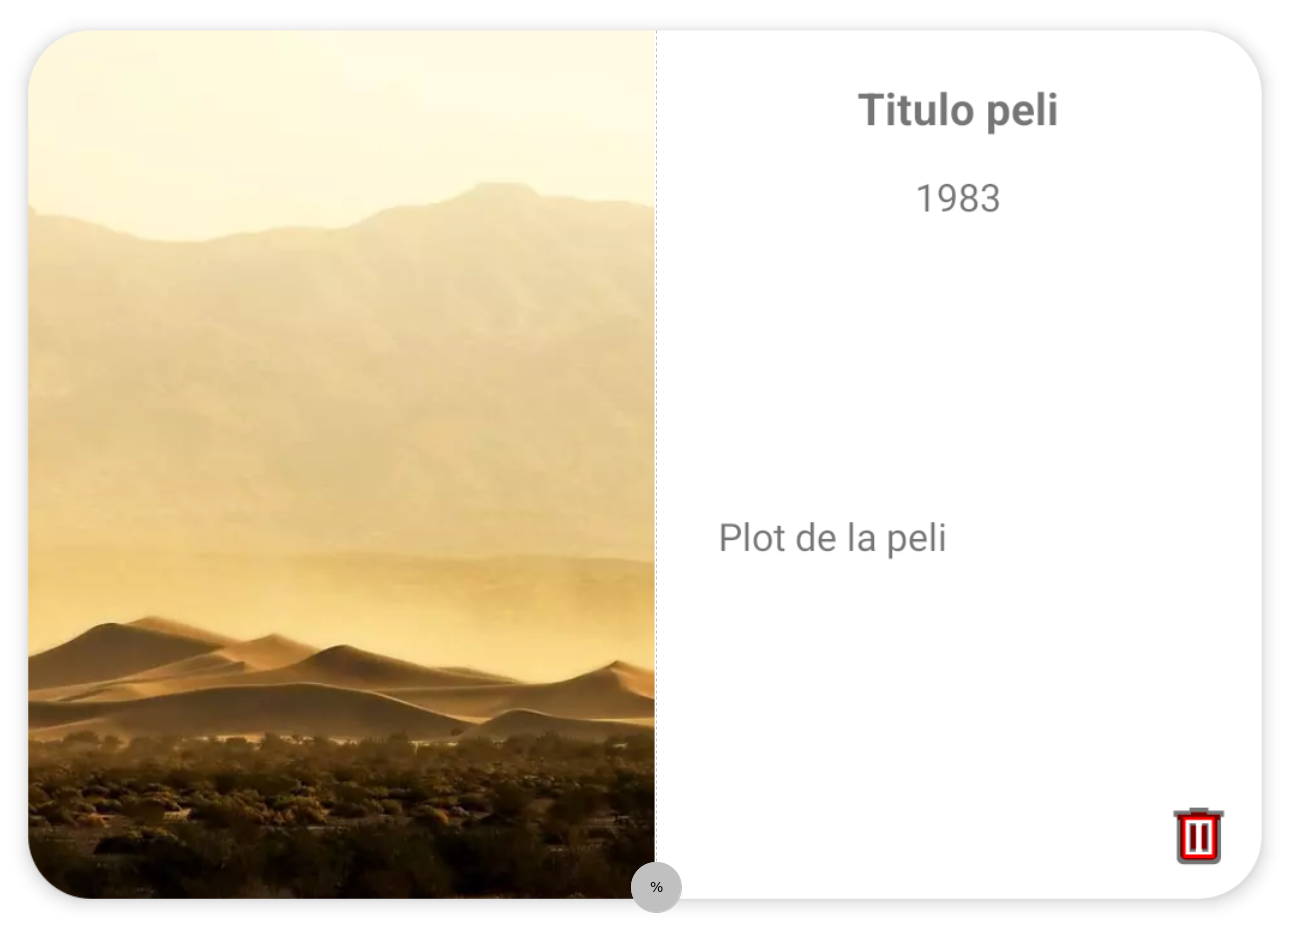
\includegraphics[width=0.6\linewidth]{img/movie_item.png}
    \vspace{-20pt}
\end{center}

Esta es la vista que en el \textbf{\textit{MovieAdapter}} se le indica al RecyclerView que debe de utilizar para \textit{bindear} los datos:

\begin{mycode}{Función que guarda el estado}{kotlin}{}
fun bind(movie: Movie) {
    nameTextView.text = movie.name
    yearTextView.text = movie.release.toString()
    plotTextView.text = movie.plot.substring(0,250) + " ..."
    Picasso.get().load(Uri.parse(movie.posterUrl))
        .placeholder(R.drawable.ic_launcher_foreground)
       .into(movieImage)
}
\end{mycode}

De esta manera, RecyclerView creará los elementos necesarios del tipo vista \textbf{movie\_item.xml}, que contendrá los datos de cada película y que mostrará por pantalla. El resultado visual final será el siguiente:

\begin{center}
    \includegraphics[width=0.5\linewidth]{img/list.png}
\end{center}


Tal como se puede ver en la imagen, cada elemento de la lista tiene el mismo aspecto visual, pero con los datos distintos, que son los obtenidos de la base de datos DataStore.

Al seleccionar un elemento de la lista, la aplicación nos enviará a otra pantalla donde veremos los datos completos de la película.

\chapter{Conclusiones}

A la hora de crear una aplicación para móvil es vital  conocer las distintas características que nos proporciona la plataforma y el lenguaje de programación que estemos utilizando. De esta manera no sólo programaremos mejor, si no que como consecuencia también conseguiremos una mejor experiencia de usuario y que esta no se vea comprometida.

También es importante conocer y hacer uso de librerías externas, que nos proporcionarán nuevas opciones que quizá la plataforma no nos ofrece, o “simplemente” nos facilitará el trabajo a la hora de utilizar características complejas.


\end{document}
